\documentclass{article}
\usepackage{lingmacros}
\usepackage[margin=1.7in]{geometry}
\usepackage{graphicx}
\graphicspath{ {./img/} }
\begin{document}
\author{Benjamin Barda, Francesco Danese, Alessandro Vecchi}
\title{\vspace{-2cm}\textbf{Self-Supervised meets Active-Learning}}
\maketitle

\section{Introduction}
\begin{flushleft}
While Data is getting generated at an ever increasing speed and can be retrieved with not much effort,
making this data useful and usable is still not a trivial task at all.
One of the main bottlenecks is the need of vast amount of labeled data, which, for a high quality dataset,
needs to be manually labeled with care, a process that requires a lot of man-hours to complete. 
This is the foundamental problem that researchers in the field of Active Learning are trying to answer. 
How can we get competitive performance with less data?
\end{flushleft}
\begin{flushleft}
The core idea of Active Learning is to get more out of the human in the loop.
But how can we do this?
Clearly is not possible to force someone to annotate faster, but what we can do is make sure 
that every sample that he labels have as much impact as possible, by selecting those with higher \emph{uncertainty} .


\begin{figure}[h]
    \centering
    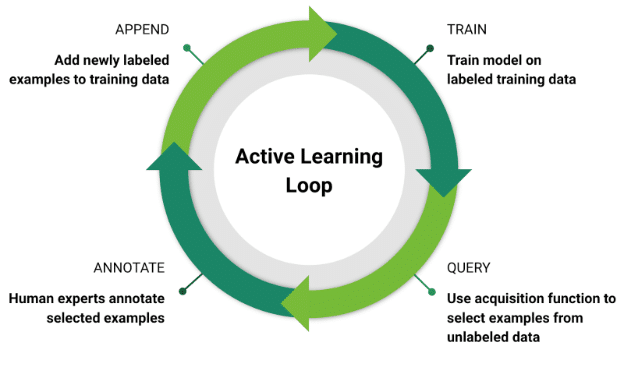
\includegraphics[scale=0.5]{AL-loop}
\end{figure}

The process is relatively simple from an overview perspective.

Starting from an existing dataset of unlabeled data we select via an acquisition 
function the \emph{most informative} samples to be presented to the oracle (a human expert for example) 
for he to annotate them and add them to the labeled dataset. We then train the model on the labeled data. 
We repeat this process until exhausting the labelling budget (time, money, ecc..).

\section{Measuring uncertainty}
\subsection{Acquisition functions}
To know how much the model is certain about the prediction it makes for a given sample, 
we need some kind of function the takes into consideration the output of the model for that particular sample.
Lets look at a few classic uncertainty acquisition functions:
\begin{enumerate}
    \item Entropy: $H(p) = - \sum{p_iLog_2(p_i)}$ where $p_i$ is the probability the model outputs for class \emph{i}, 
    refering for instance to the last softmax layer of a NeuralNet.
    H will grow as the probabilities p tend to be more uniform, and will shrink when fewer of the categories tend to get higher values.
    \item Variation ratio: $1 - max(p)$
    \item The difference between the largest output from the model, and the second largest output.
    \item In SVMs: the distance of a point from the hyperplane.
\end{enumerate}
\subsection{Query by Committee QBC}
Another concept from classical active learning papers, is QBC. 
The idea here is that instead of measuring the uncertainty of a single model, 
we can train an ensemble of many different models (maybe with different seeds, 
or hyper-parameters, or structures). Then for a given image, 
we can check if the output changes a lot between models. If it does, 
it means the models aren’t very consistent about this image, 
and some of them aren’t doing a good job on this image.
\section*{Active Learning: Not only one way}
There are three main approaches to the problem :
\begin{itemize}
    \item Stream based selective sampling
    \item Pool-Based sampling
    \item Membership query synthesis
\end{itemize}
In this project we investigare Pool-Based sampling but a ìn overview of the various methods this article might be a good starting point.

\subsection*{Our approach}
Our approach can be divided in two main steps:
\begin{itemize}
    \item Pretrain
    \item Active learning loop
\end{itemize}

\subsection*{Pretrain}
This is a crucial part of the method proposed, in fact the quality of the features learned 
during this phase have a great impact on the final performnace, 
so we put great consideration in selecting the appropiate pretext task.

The one thing that remained constant during all of our experiments 
were was the choice of the architechture. 
We decided to use a Residual Network for two reasons:
\begin{enumerate}
    \item Low number of learnable parameters
    \item Proved history of great performance on CIFAR10, the dataset we chose for this project.
\end{enumerate}
During the first phase of the project we considered using the non constrastive task 
described in SimSiam. Even though the quality of the features were excellent 
we faced the problem of limited resources in terms of computing and time, 
and since to have an effective pretrain we would need to run at least 800 epochs 
we decided to discard this option.
\end{flushleft}
\begin{flushleft}
We then resorted to a simpler task, more specifically rotation prediction, 
as described in the RotNet paper. The task is pretty straight forward. 
Given an unlabeled image, we rotate it by 90, 180 and 270 degreees, 
associating to each rotation a label (0 for no rotation, 1 for 90deg rotation, ecc). 
We then train a classifier over the rotated images. 
\end{flushleft}
\begin{flushleft}
The idea is that the network is forced to focus on important features 
of the image in order to recognize the rotation thus learning usefull features 
rappresentaions. The big advantage over the SimSiam approach is the realative low number of epochs it needs. 
In fact around 100 epochs are needed to have an effective pretrain, allowing us to complete the training in a 
single colab session in less than 2 hours.
\end{flushleft}
\end{document}